% !Mode:: "TeX:UTF-8"
% !TEX program  = xelatex
\section{Applications}\label{S:applications}
\subsection{Solution to Article Title}
From the definition of quadratic equation in Section~\ref{S:quadratic}, we can finally answer the question, \emph{what Angle Should We Throw a Football for Maximum Range?}

Firstly, we establish a rectangular coordinate system, as shown in Figure~\ref{F:parabolic-throwing}. We denote $\theta$ as shot angle, $V$ as initial velocity, $g$ as gravity, $S$ as distance, $t$ as time.

\begin{figure}
    \centering
    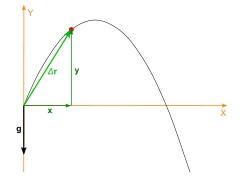
\includegraphics[width=.45\textwidth]{figures/quadratic_equation-3.png}
    \caption{Displacement and coordinates of parabolic throwing}\label{F:parabolic-throwing}
\end{figure}

Then, we have both horizontal and vertical velocity,
\begin{equation}\label{E:solution-1}
    \begin{cases}
        V_x &= V\cos(\theta) \\
        V_y &= V\sin(\theta) - gt
    \end{cases}
\end{equation}

Therefore, we have both horizontal and vertical distance at time $t$,
\begin{equation}\label{E:solution-2}
    \begin{cases}
        S_x &= V\cos(\theta)t \\
        S_y &= V\sin(\theta)t - \frac{1}{2} gt^2
    \end{cases}
\end{equation}

From Equation~\eqref{E:solution-1} and Equation~\ref{E:solution-1}, we can find all of the coordinate $(S_x, S_y)$ with angle $\theta$. From Equation~\eqref{E:solution-2}, we have $t=\tfrac{2V\sin(\theta)}{g}$, then we substitute the expression of $t$ back to the $S_y$, we have the quadratic equation
\begin{equation}\label{E:solution-3}
    S_y = \tan(\theta)S_x - \frac{g}{2V^2\cos^2(\theta)}S_x^2.
\end{equation}

From Equation~\eqref{E:quadratic-formula}, we can solve this quadratic equation, the solutions are $0$ and $\tfrac{2V^2}{g}\sin(\theta)$. Obviously, $0$ is the initial position, then the football will land at $\tfrac{2V^2}{g}\sin(\theta)$, that is, $\tfrac{V^2}{g}\sin(2\theta)$.

According to knowledge of trigonometric functions, we have the maximum range of the football is $\tfrac{V^2}{g}$, which is taken at $\theta=45$.


\subsection{Simulation of Projectile Motion}
You can use quadratic equation to simulate projectile motion, which can solve free fall problems. If you are familiar with \texttt{Python}, you can use \texttt{Python} to draw the pictures of trajectories, and you will find it easy to use Python to solve quadratic equations, especially in symbolic calculations. And the code is in Appendix~\ref{A:python}.
